\chapter{不可逆变化}\label{ch:g5:irreversible-changes}

把一个鸡蛋打进热锅里。几秒钟内，清亮、稀薄的
蛋清变得坚硬发白，蛋黄也凝固变稠。把锅从炉灶上拿下，
让鸡蛋冷却，再放进冰箱：它永远不会再变回生鸡蛋。有些变化可以恢复，有些则不能。
分辨它们，
是化学学习的第一步。

\begin{recall}
溶于水的固体并没有消失：水干了以后，
固体会留下来（见\cref{ch:g2:mixing-and-dissolving}）。
\omterm{def:g4:what-a-fire-needs:burning}{燃烧}会生成新的物质——灰烬、烟、二氧化碳和水蒸气——
\omterm{def:g4:what-a-fire-needs:fuel}{燃料}也就永远消失了（见\cref{ch:g4:what-a-fire-needs}）。
\end{recall}

\begin{omfigure}
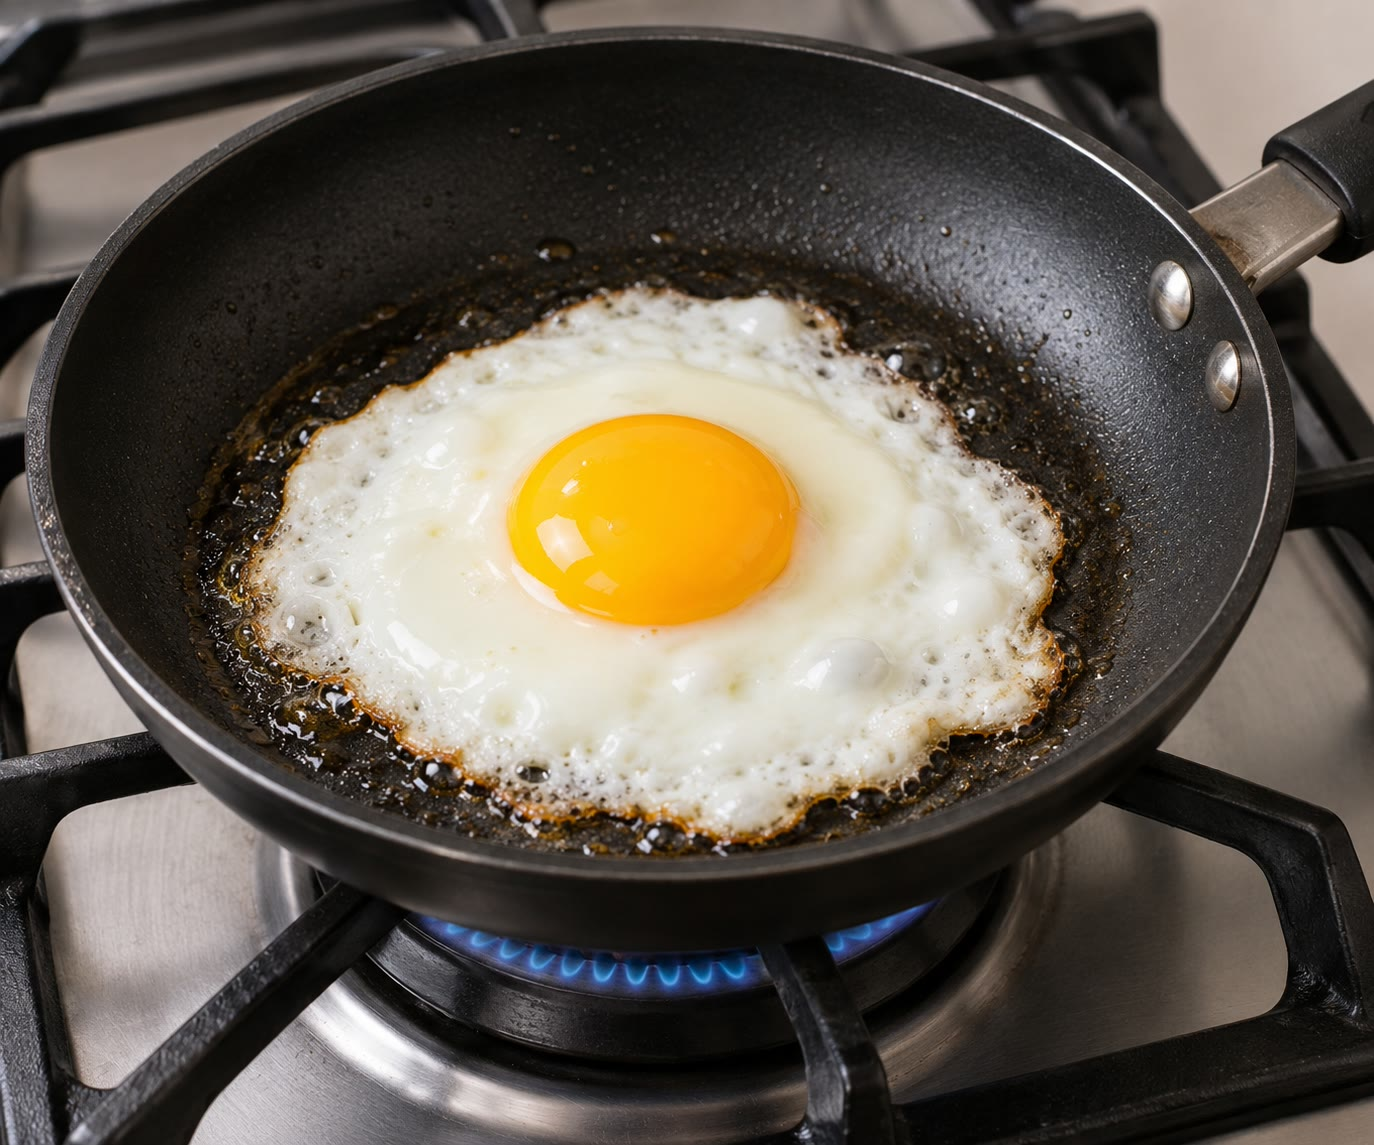
\includegraphics[width=0.55\linewidth]{images/book1/ai/g5-egg-frying.jpg}

{\small 煎蛋：清亮的蛋清已经变得坚硬发白，
再也无法复原。}
\end{omfigure}

\section{可逆变化}

\begin{definition}[可逆变化]\label{def:g5:irreversible-changes:reversible}
称\emph{可逆变化}\index{可逆变化}为能够
被逆转、从而恢复到最初状态的变化。
\end{definition}

\begin{example}[溶解与蒸发]\label{ex:g5:irreversible-changes:dissolve}
把糖搅拌进水中，糖会\omterm{def:g2:mixing-and-dissolving:dissolve}{溶解}。让水\omterm{def:g3:separating-mixtures:evaporate}{蒸发}，
糖会重新出现：还是原来的糖，依然一样甜。\omterm{def:g2:mixing-and-dissolving:dissolve}{溶解}
是一种\omterm{def:g5:irreversible-changes:reversible}{可逆变化}。
\end{example}

\begin{example}[冰与水]\label{ex:g5:irreversible-changes:ice}
把一块冰放在温热的盘子上，会熔化成水；把水放进
冷冻室里，水又会变回冰。熔化和凝固都是
\omterm{def:g5:irreversible-changes:reversible}{可逆变化}。（水为什么会熔化和凝固，在物理书中讲。）
\end{example}

\begin{example}[混合]\label{ex:g5:irreversible-changes:mix}
与砾石\omterm{def:g2:mixing-and-dissolving:mix}{混合}的沙子可以用筛子重新分开；浑浊的水
可以\omterm{def:g3:separating-mixtures:filter}{过滤}。\omterm{def:g2:mixing-and-dissolving:mix}{混合}是\omterm{def:g5:irreversible-changes:reversible}{可逆变化}：没有生成新物质，
各部分都能被分离（见\cref{ch:g3:separating-mixtures}）。
\end{example}

\section{不可逆变化}

\begin{definition}[不可逆变化与化学变化]\label{def:g5:irreversible-changes:chemical-change}
称\emph{不可逆变化}\index{不可逆变化}为
不能简单恢复的变化。大多数此类变化中，会出现
原本不存在的新物质：这类变化称为
\emph{化学变化}\index{化学变化}。
\end{definition}

\begin{example}[六种化学变化]\label{ex:g5:irreversible-changes:six}
\begin{itemize}
  \item \textbf{煮鸡蛋}：稀薄、透明的蛋清变成
        坚硬发白。
  \item \textbf{烤蛋糕}：稀薄的面糊变成
        松软的蛋糕，外皮呈褐色，并带有新的气味。
  \item \textbf{\omterm{def:g4:what-a-fire-needs:burning}{燃烧}}：木材变成
        灰烬、烟、二氧化碳和水蒸气。
  \item \textbf{生锈}：露在雨中的光亮铁器变成
        覆盖着一层橙褐色的片状物质——铁锈。
  \item \textbf{牛奶变酸}：放置数天后，牛奶变稠、
        结块，并散发出酸味。
  \item \textbf{切开的苹果变褐}：浅色果肉在
        \omterm{def:g4:air-a-mixture-of-gases:air}{空气}中一小时内就变成褐色。
\end{itemize}
每一种情况下都生成了新物质，而且无法
简单地恢复到最初的状态。
\end{example}

\begin{omfigure}
\begin{minipage}[t]{0.48\linewidth}\centering
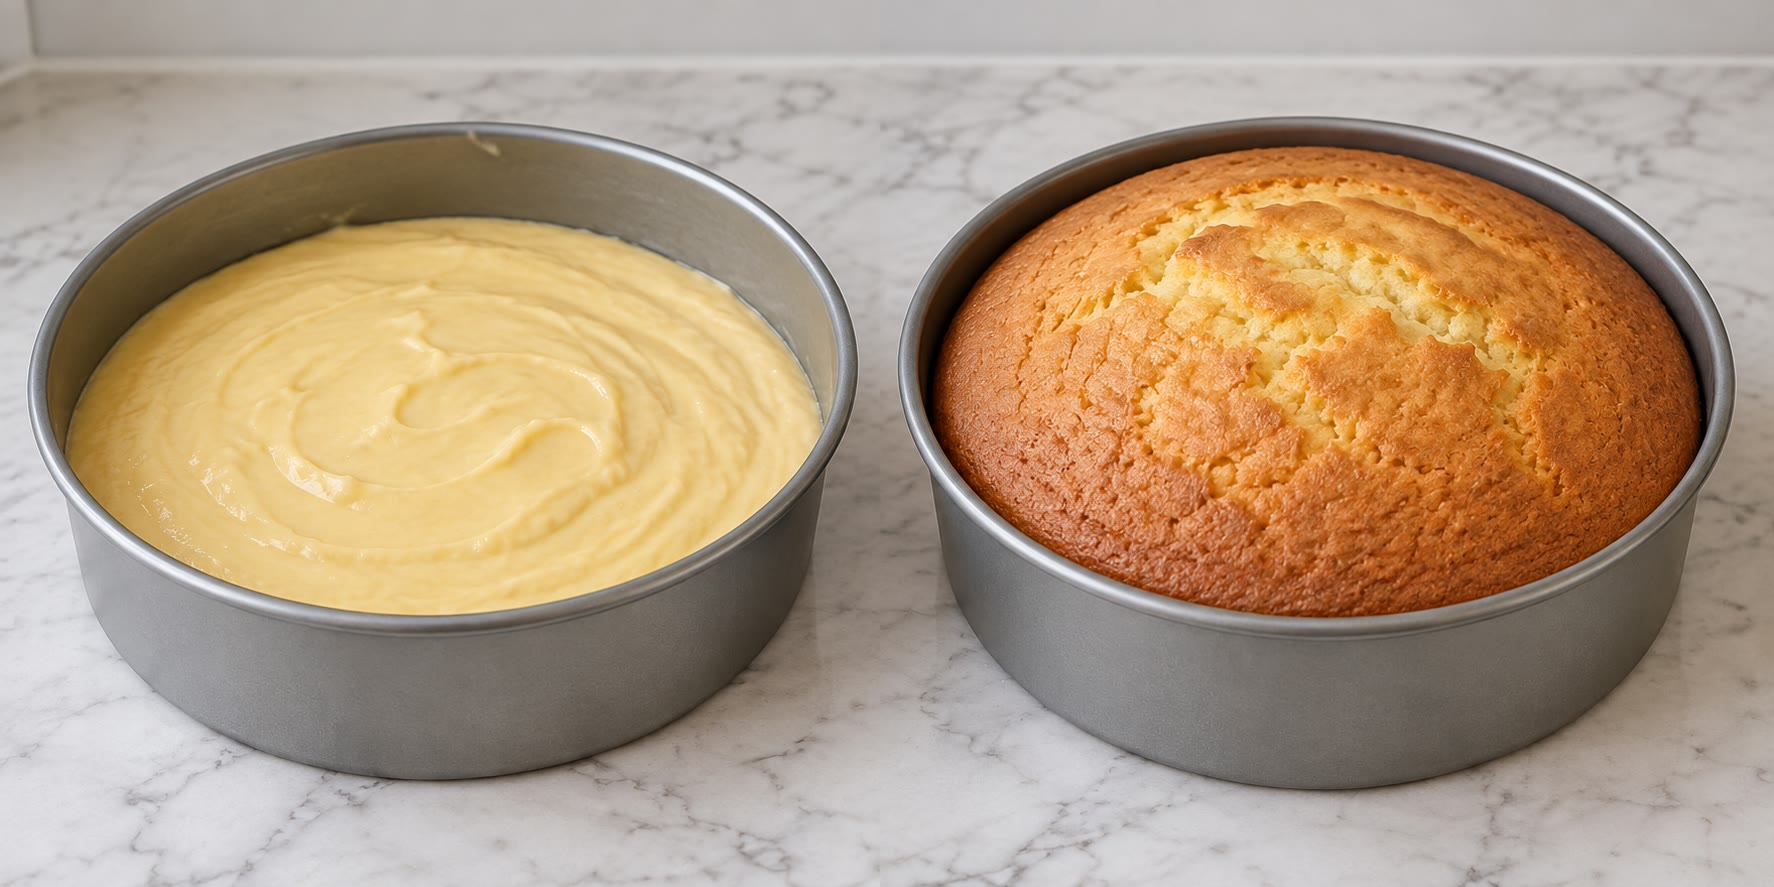
\includegraphics[width=\linewidth,height=4.6cm,keepaspectratio]{images/book1/ai/g5-cake-before-after.jpg}

{\small 烤前为面糊，烤后为蛋糕：烘烤不可逆转。}
\end{minipage}\hfill
\begin{minipage}[t]{0.48\linewidth}\centering
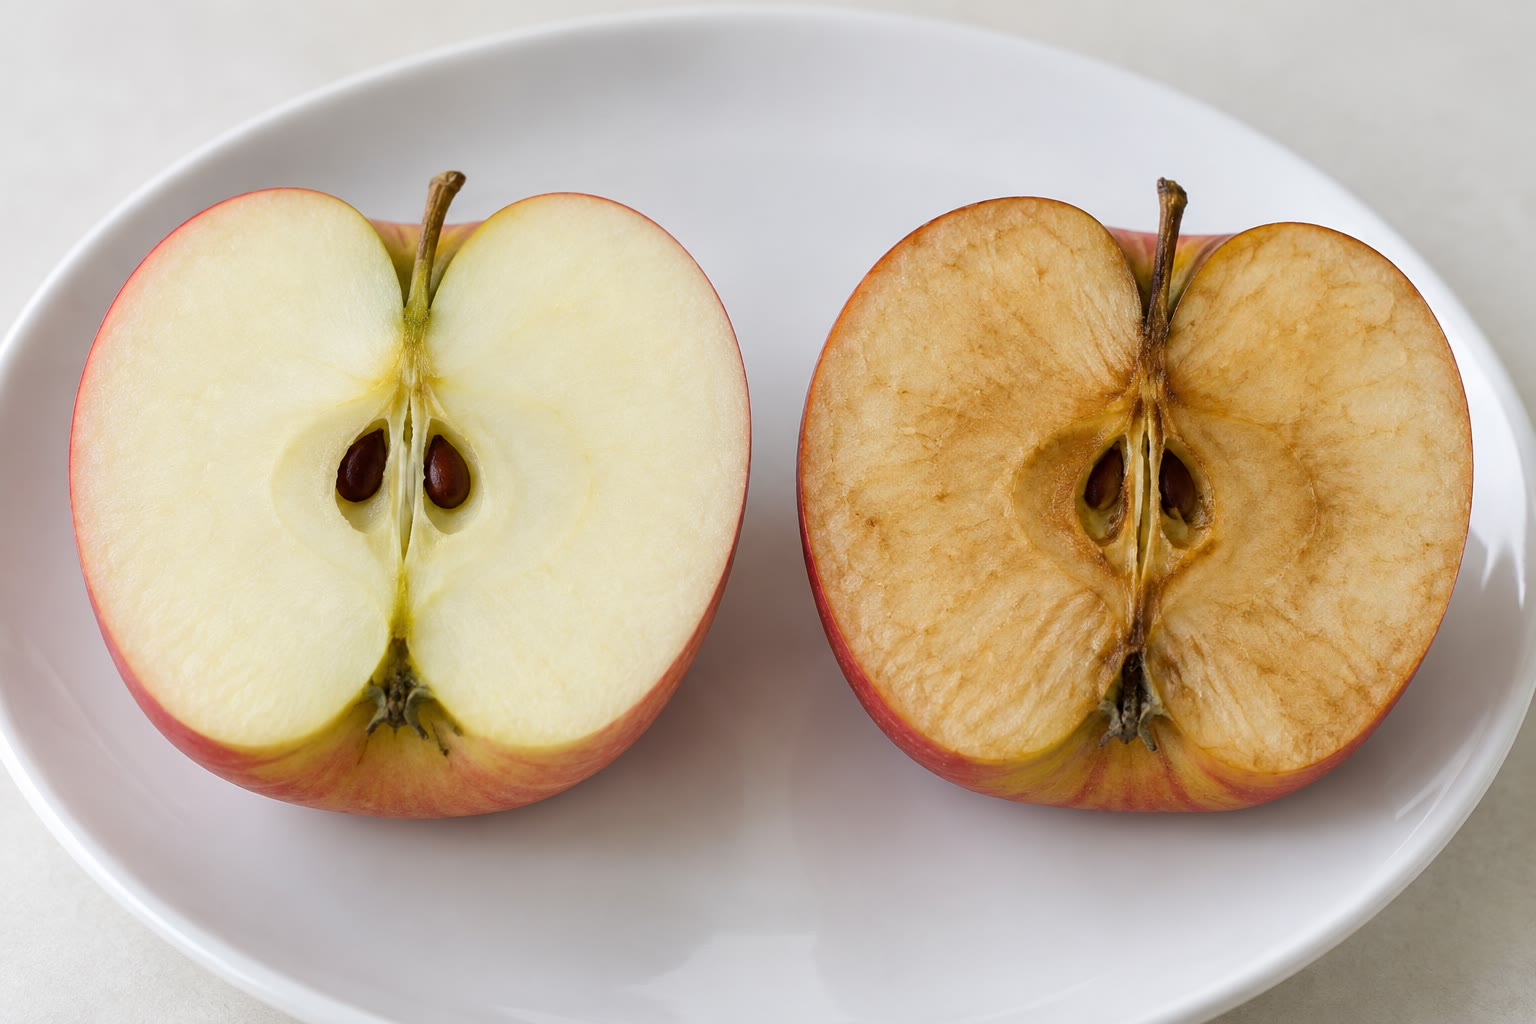
\includegraphics[width=\linewidth,height=4.6cm,keepaspectratio]{images/book1/ai/g5-apple-browning.jpg}

{\small 刚切开的一半苹果，与在\omterm{def:g4:air-a-mixture-of-gases:air}{空气}中放置一小时的另一半。}
\end{minipage}
\end{omfigure}

\begin{omfigure}
\begin{tikzpicture}[font=\small]
  \node[font=\small\bfseries, omDef] at (2.7,4.6) {可逆};
  \node[font=\small\bfseries, omProp] at (9.6,4.6) {不可逆};
  \draw[black!30] (6.1,4.9) -- (6.1,-0.3);
  % reversible pairs
  \foreach \y/\a/\b in {3.6/{糖 + 水}/{糖水}, 2.0/{冰}/{液态水},
                        0.4/{沙子 + 砾石}/{混合物}} {
    \node[draw=omDef, fill=omDef!6, rounded corners=2pt, minimum width=2.3cm,
      minimum height=0.8cm] at (0.9,\y) {\a};
    \node[draw=omDef, fill=omDef!6, rounded corners=2pt, minimum width=2.3cm,
      minimum height=0.8cm] at (4.6,\y) {\b};
    \draw[->, thick, omDef] (2.3,\y+0.12) -- (3.25,\y+0.12);
    \draw[<-, thick, omDef] (2.3,\y-0.12) -- (3.25,\y-0.12);
  }
  % irreversible ones
  \foreach \y/\a/\b in {3.6/{生鸡蛋}/{熟鸡蛋}, 2.0/{木头}/{灰、烟和气体},
                        0.4/{铁}/{铁锈}} {
    \node[draw=omProp, fill=omProp!6, rounded corners=2pt, minimum width=2.0cm,
      minimum height=0.8cm] at (7.6,\y) {\a};
    \node[draw=omProp, fill=omProp!6, rounded corners=2pt, minimum width=2.9cm,
      minimum height=0.8cm] at (11.5,\y) {\b};
    \draw[->, thick, omProp] (8.8,\y) -- (9.85,\y);
  }
\end{tikzpicture}

{\small 左图：\omterm{def:g5:irreversible-changes:reversible}{可逆变化}，双箭头表示它们可以
双向进行。右图：\omterm{def:g5:irreversible-changes:chemical-change}{化学变化}，只能单向进行。}
\end{omfigure}

\section{出现新物质的线索}

\begin{method}[是化学变化吗？寻找线索]\label{met:g5:irreversible-changes:clues}
出现新物质时，往往有以下线索之一：
\begin{enumerate}
  \item 出现新的\textbf{颜色}（烤面包片变成的褐色）；
  \item 未经加热，液体中出现气体的
        \textbf{气泡}（醋倒在小苏打上）；
  \item 出现新的\textbf{气味}（变酸的牛奶、烤焦的面包）；
  \item 放出\textbf{热量或光}（\omterm{def:g4:what-a-fire-needs:burning}{燃烧}的蜡烛）；
  \item 澄清的液体中\textbf{出现固体}，或
        形成块状物（牛奶凝结）。
\end{enumerate}
仅凭一条线索可能导致误判：水沸腾时冒泡，但
并未生成新物质——冒出的是水的蒸气，
蒸气冷却后水又会回来。多找几条线索，并问一问：能否复原？
\end{method}

\begin{omfigure}
\begin{tikzpicture}[font=\small]
  \foreach \k/\t in {0/{新的颜色}, 1/{气泡}, 2/{新的气味},
                     3/{发热或发光}, 4/{出现固体}} {
    \begin{scope}[xshift=\k*3.2cm]
      \draw[omProp, line width=0.8pt, fill=omProp!5] (0,0) circle (1.0);
      \node[anchor=north, align=center] at (0,-1.15) {\t};
    \end{scope}
  }
  % 1: colour, a slice of toast half brown
  \fill[yellow!20, draw=brown!60] (-0.55,-0.5) rectangle (0.55,0.55);
  \fill[brown!55] (0,-0.5) rectangle (0.55,0.55);
  % 2: bubbles in a beaker
  \begin{scope}[xshift=3.2cm]
    \pic[transform shape, scale=0.45] at (0,-0.55) {beaker={0.7}{omWater!80}};
    \foreach \x/\y in {-0.15/-0.2,0.1/0.05,-0.05/0.25,0.18/-0.35,-0.2/0.15}
      \draw[black!55] (\x,\y) circle (0.05);
  \end{scope}
  % 3: smell, wavy lines
  \begin{scope}[xshift=6.4cm]
    \foreach \x in {-0.35,0,0.35} \draw[black!55, line width=0.8pt, decorate,
      decoration={snake, amplitude=1.5pt, segment length=6pt}] (\x,-0.6) -- (\x,0.6);
  \end{scope}
  % 4: a flame
  \begin{scope}[xshift=9.6cm]
    \fill[orange!80] (0,-0.6) .. controls (-0.45,-0.05) and (-0.15,0.35) .. (0,0.7)
      .. controls (0.15,0.35) and (0.45,-0.05) .. (0,-0.6);
    \fill[yellow!80] (0,-0.45) .. controls (-0.2,-0.1) and (-0.08,0.15) .. (0,0.3)
      .. controls (0.08,0.15) and (0.2,-0.1) .. (0,-0.45);
  \end{scope}
  % 5: solid settling in a test tube
  \begin{scope}[xshift=12.8cm]
    \pic[transform shape, scale=0.4] at (0,-0.65) {testtube={0.75}{omWater!80}};
    \fill[white, draw=black!40] (-0.08,-0.62) rectangle (0.08,-0.5);
    \foreach \x/\y in {-0.04/-0.3,0.04/-0.1,0/0.1} \fill[black!35] (\x,\y) circle (0.03);
  \end{scope}
\end{tikzpicture}

{\small \omterm{def:g5:irreversible-changes:chemical-change}{化学变化}可能发生的五条线索。}
\end{omfigure}

\begin{inthelab}[醋与小苏打]
老师取一勺白色粉末状的小苏打，放在
烧杯底部，再倒入一些醋。\omterm{def:g2:mixing-and-dissolving:mix}{混合}物立即嘶嘶作响、冒出泡沫：
放出了气体，这是\omterm{def:g5:irreversible-changes:chemical-change}{化学变化}的线索。嘶嘶声停止后，
小苏打已经消失，
无法通过干燥将其复原。
\end{inthelab}

\begin{omfigure}
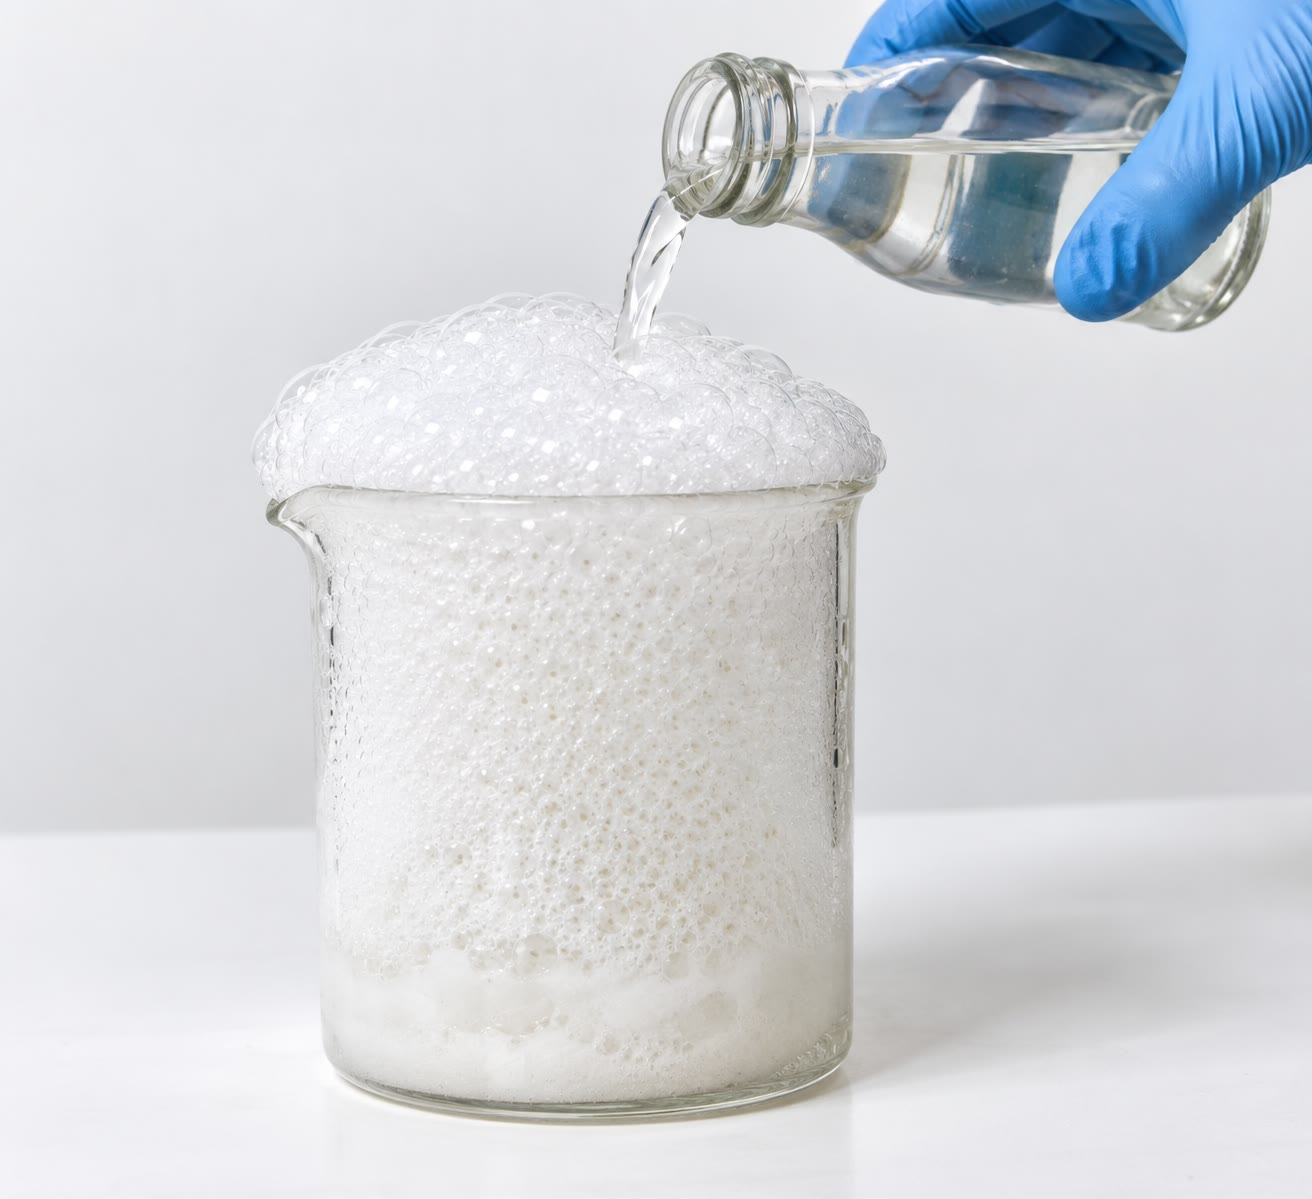
\includegraphics[width=0.5\linewidth]{images/book1/ai/g5-baking-soda-lab.jpg}

{\small 醋与小苏打反应：放出气体。}
\end{omfigure}

\section{有利和有害的变化}

\begin{proposition}[身边的化学变化]\label{prop:g5:irreversible-changes:around}
许多\omterm{def:g5:irreversible-changes:chemical-change}{化学变化}是有益的：烹饪食物、烘焙面包、
\omterm{def:g4:what-a-fire-needs:burning}{燃烧}燃气为房屋供暖，石膏或水泥凝固变硬。另一些则造成损害：
铁生锈、食物变质、木材腐烂。这些变化无法逆转，
但可以减缓它们的进程：
\begin{itemize}
  \item 食物放在冰箱的低温中可以保存更久；
  \item 油漆或一层油膜可以隔绝\omterm{def:g4:air-a-mixture-of-gases:air}{空气}和水，保护铁；
  \item 切开的苹果撒上柠檬汁，变褐色的速度更慢。
\end{itemize}
\end{proposition}

\begin{omfigure}
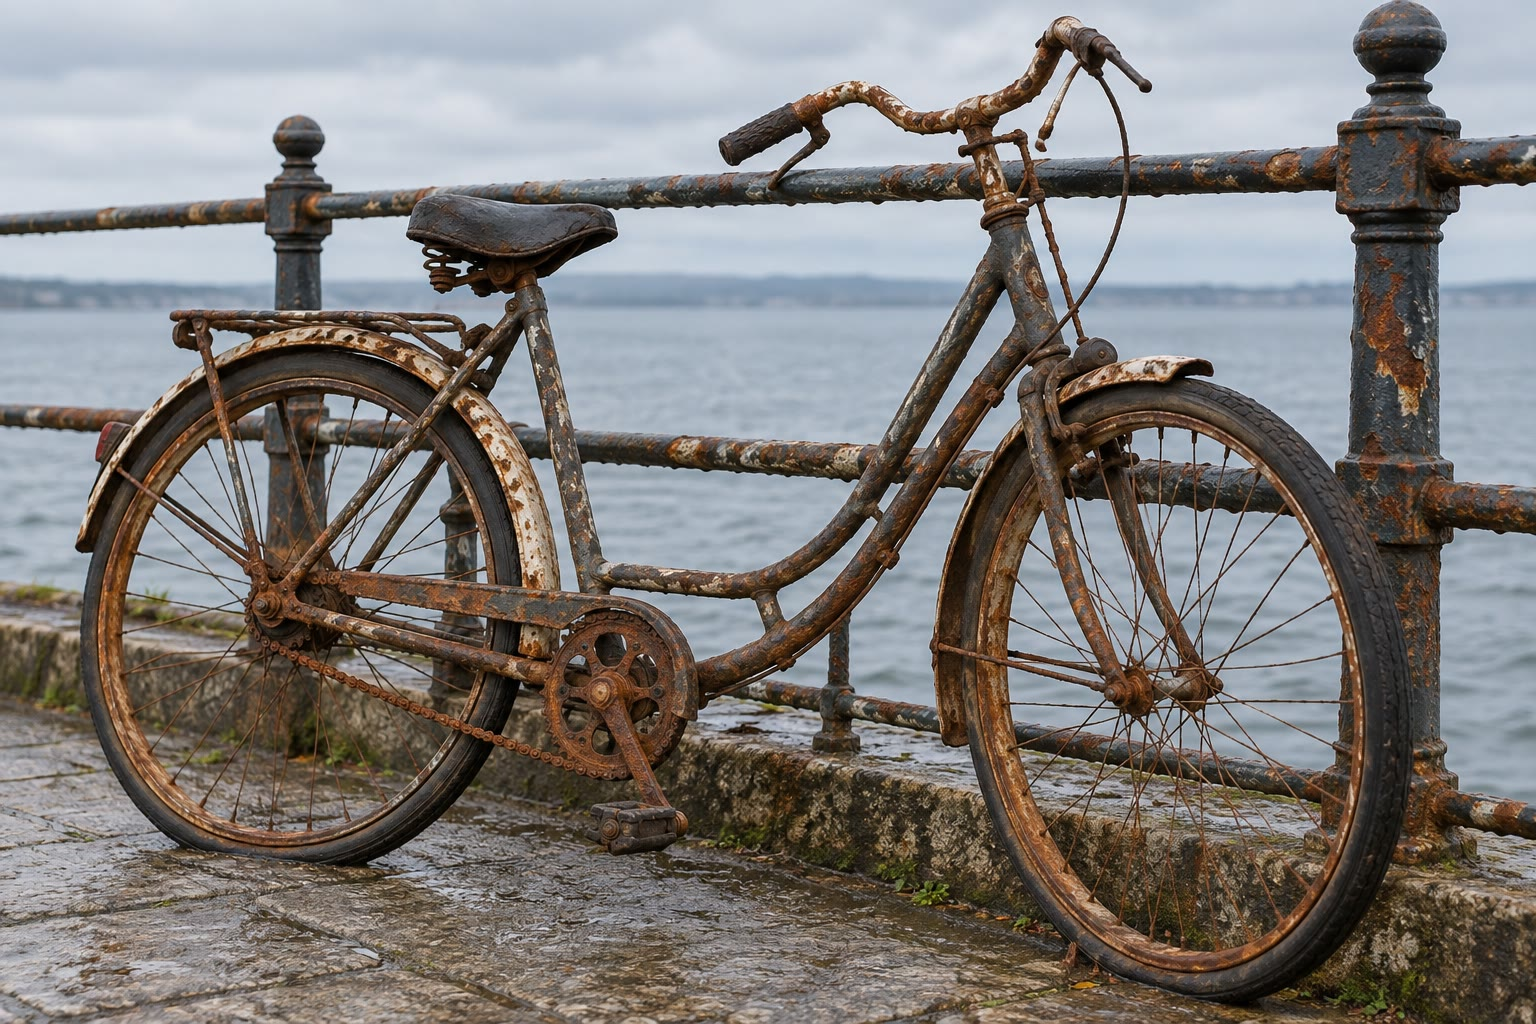
\includegraphics[width=0.55\linewidth]{images/book1/ai/g5-rusty-bicycle.jpg}

{\small 一辆自行车长年露天放置在雨中：铁已经生锈。}
\end{omfigure}

\begin{remark}[无法逆转，但并不简单]\label{rem:g5:irreversible-changes:not-simply}
“无法逆转”是指没有简单的办法可以回到原状，
例如冷却或干燥。化学家有时可以把铁锈变回铁，
但需要借助熔炉和新的物质：这仍然是另一个\omterm{def:g5:irreversible-changes:chemical-change}{化学变化}，
而不是简单地逆转。
\end{remark}

\section{练习}

\begin{exercise}[$\star$]\label{exo:g5:irreversible-changes:1}
判断下列各变化是否可以逆转：熔化巧克力、\omterm{def:g4:what-a-fire-needs:burning}{燃烧}
火柴、盐溶于水、烤面包。
\end{exercise}

\begin{exercise}[$\star$]\label{exo:g5:irreversible-changes:2}
什么是\omterm{def:g5:irreversible-changes:chemical-change}{化学变化}？请举出两个厨房里的例子。
\end{exercise}

\begin{exercise}[$\star$]\label{exo:g5:irreversible-changes:3}
盐\omterm{def:g2:mixing-and-dissolving:dissolve}{溶解}在水中。怎样才能把盐重新取回？
\omterm{def:g2:mixing-and-dissolving:dissolve}{溶解}是\omterm{def:g5:irreversible-changes:reversible}{可逆变化}吗？
\end{exercise}

\begin{exercise}[$\star$]\label{exo:g5:irreversible-changes:4}
牛奶变酸时，你注意到\omterm{def:g5:irreversible-changes:chemical-change}{化学变化}的哪种迹象？
请说出两个。
\end{exercise}

\begin{exercise}[$\star$]\label{exo:g5:irreversible-changes:5}
看一看这幅分为两栏的图，哪些变化带有双箭头？
双箭头表示什么意思？
\end{exercise}

\begin{exercise}[$\star$]\label{exo:g5:irreversible-changes:6}
为什么要给自行车链条上油？
油能减慢哪一种\omterm{def:g5:irreversible-changes:chemical-change}{化学变化}？
\end{exercise}

\begin{exercise}[$\star$]\label{exo:g5:irreversible-changes:7}
把醋倒在小苏打上时会冒出气泡，这是哪一种迹象？
\end{exercise}

\begin{exercise}[$\star$]\label{exo:g5:irreversible-changes:8}
请各举一个有益的\omterm{def:g5:irreversible-changes:chemical-change}{化学变化}和一个有害的\omterm{def:g5:irreversible-changes:chemical-change}{化学变化}。
\end{exercise}

\begin{exercise}[$\star$]\label{exo:g5:irreversible-changes:9}
为什么要把牛奶放在冰箱里？
\end{exercise}

\begin{exercise}[$\star\star$]\label{exo:g5:irreversible-changes:10}
水沸腾时会冒泡。沸腾是否为\omterm{def:g5:irreversible-changes:chemical-change}{化学变化}？请说明
为什么仅凭一种迹象是不够的。
\end{exercise}

\begin{exercise}[$\star\star$]\label{exo:g5:irreversible-changes:11}
汤姆说：“蜡烛\omterm{def:g4:what-a-fire-needs:burning}{燃烧}时，蜡就像冰一样融化掉了。”
用两个迹象解释为什么\omterm{def:g4:what-a-fire-needs:burning}{燃烧}蜡烛是\omterm{def:g5:irreversible-changes:chemical-change}{化学变化}，
而不只是熔化。
\end{exercise}
